% !TEX root =  main.tex
%%%%%%%%%%%%%%%%%%%%%%%%%%%%%%%%%%%%%
%%%%%%%%%%%%%%%%%%%%%%%%%%%%%%%%%%%%%
\vspace{-0.2cm}
\section{Experiments}
\label{experiments}
\begin{table}[t!]
\centering
\scriptsize
\setlength{\tabcolsep}{3pt}

\begin{minipage}[t]{0.35\linewidth}
\centering
\begin{tabular}{lccc}
\toprule
\textbf{Method} & \textbf{L2-7B} & \textbf{L3-8B} & \textbf{Q3-8B} \\
\midrule
\textbf{\method} & \textbf{96} & \textbf{98} & \textbf{100} \\
Self-Refine   & 4  & 14 & 58 \\
AdvReasoning  & 60 & 88 & 80 \\
AutoDAN-Turbo & 36 & 62 & 83 \\
PAIR          & -  & 75 & 47 \\
UJA           & -  & 72 & 63 \\
\bottomrule
\end{tabular}
\subcaption{HarmBench ASR (\%).}
\label{tab:harmbench_asr}
\end{minipage}\hfill
\begin{minipage}[t]{0.38\linewidth}
\centering
\begin{tabular}{lccc}
\toprule
\textbf{Method} & \textbf{L2-7B} & \textbf{L3-8B} & \textbf{Q3-8B} \\
\midrule
\textbf{\method}
& \begin{tabular}[t]{@{}c@{}}\textbf{0.58}\\[-1pt]$\pm$ 0.0059\end{tabular}
& \begin{tabular}[t]{@{}c@{}}\textbf{0.59}\\[-1pt]$\pm$ 0.0082\end{tabular}
& \begin{tabular}[t]{@{}c@{}}\textbf{0.85}\\[-1pt]$\pm$ 0.0079\end{tabular} \\
AutoDAN-Turbo & 0.12 & 0.23 & - \\
PAIR          & 0.05 & 0.12 & - \\
TAP           & 0.04 & 0.13 & - \\
PAP-top5      & 0.10 & 0.08 & - \\
\bottomrule
\end{tabular}
\subcaption{StrongREJECT judge score.}
\label{tab:strongreject_score}
\end{minipage}\hfill
\begin{minipage}[t]{0.22\linewidth}
\centering
\begin{tabular}{lc}
\toprule
\textbf{Metric} & \textbf{Value} \\
\midrule
Precision   & 0.9139 \\
Recall      & 0.9324 \\
Specificity & 0.7500 \\
F1-score    & 0.9231 \\
Accuracy    & 0.8850 \\
\bottomrule
\end{tabular}
\subcaption{Judge model vs human agreement.}
\label{tab:judge_human_metrics}
\end{minipage}

\caption{\textbf{Performance comparison with baseline red-teaming methods on open-weight models.}
Left: HarmBench ASR on open-weight target models.
Middle: StrongREJECT judge scores.
Right: Agreement between the judge model and human majority vote.}
\end{table}
\begin{figure}
\begin{subfigure}[t]{0.36\linewidth}
    \centering
    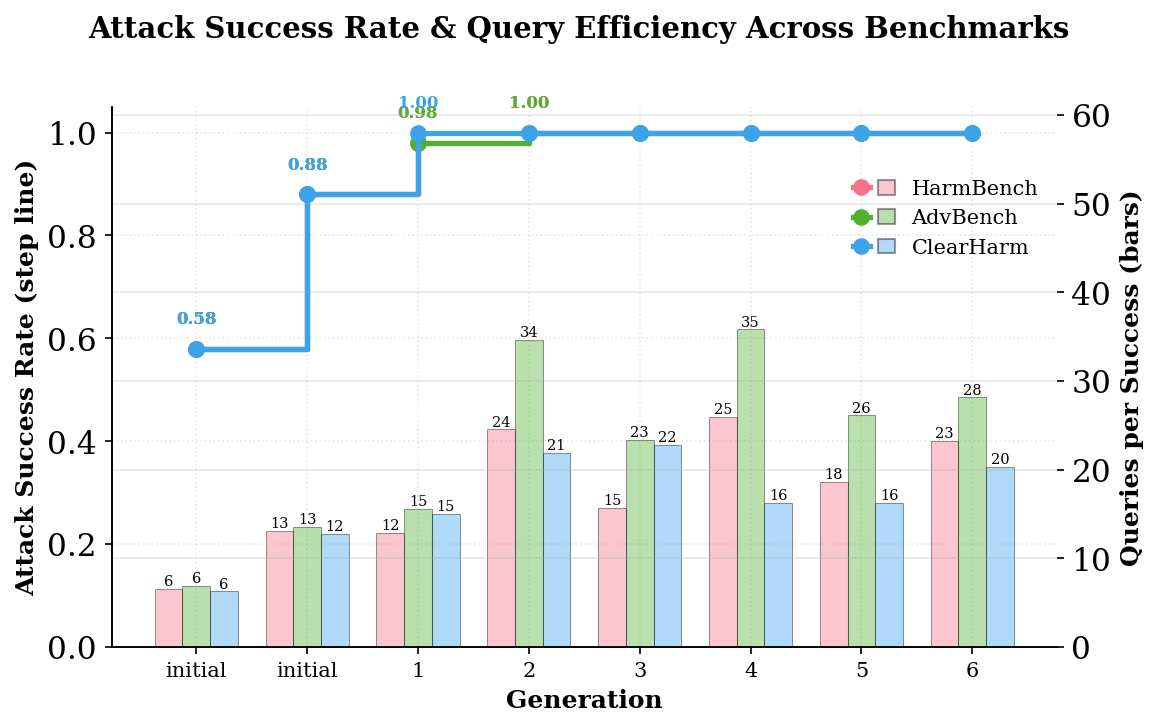
\includegraphics[width=\linewidth]{figure/Attack_Success_Rate_Query_Efficiency_Across_Benchmarks.png}
\end{subfigure}\hfill
\begin{subfigure}[t]{0.62\linewidth}
    \centering
    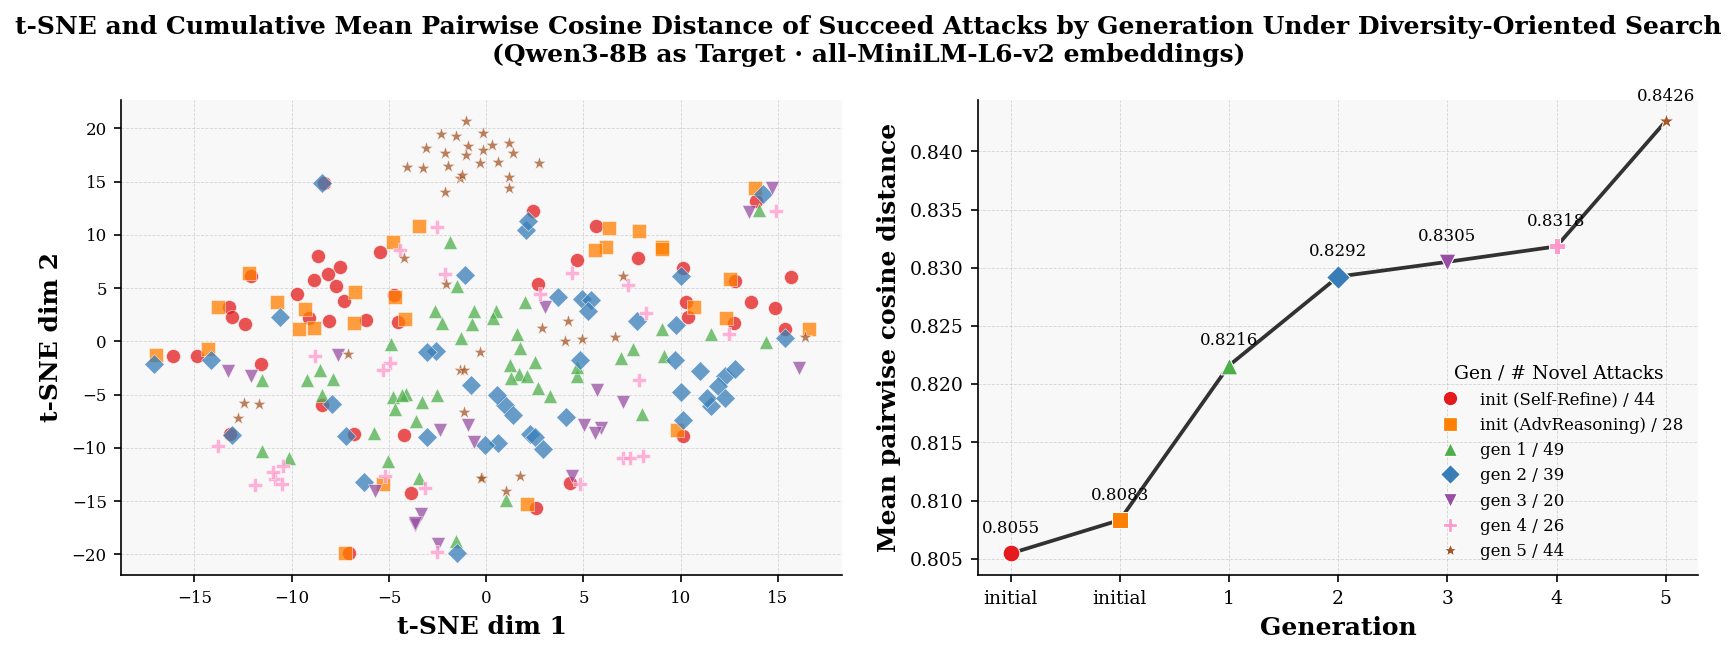
\includegraphics[width=\linewidth]{figure/tsne_and_cumulative_pairwise_distance_by_generation.png}
\end{subfigure}
\caption{\textbf{Left: Performance on open-weight models across benchmarks.} The systems designed by \method~outperform the archive and hand-designed baseline methods, showing high query efficiency and robustness across benchmark sets. \textbf{Middle + Right: Diversity trend of succeeded attacks under diversity-oriented search.} Under diversity-oriented search, successful attacks spread progressively across the embedding space, with cumulative mean pairwise cosine distance increasing monotonically.}
\vspace{-0.5cm}
\label{fig: across benchmark}
\label{fig: diversity search}
\end{figure}

\subsection{Implementation}
\label{expr:implementation}

During the evolutionary stage, we use GPT-5-2025-08-07 as the meta agent to design candidate red-teaming systems given its strong capability for system-level design. To ensure stable, reliable access to the target model and enable direct comparison with prior baselines, we use locally-hosted Llama-2-7B \citep{touvron2023llama2openfoundation}, Llama-3-8B \citep{llama3modelcard}, and Qwen3-8B \citep{qwen3technicalreport} as the target models, HarmBench-Llama-2-13b-cls as the judge function, and intention-target pairs are drawn from the HarmBench Standard dataset \citep{mazeika2024harmbench}. We run the evolutionary process under three settings: (1) Mixtral-8x7B \citep{jiang2024mixtral} attacker targeting Llama-2-7B, (2) Mixtral-8x7B attacker targeting Llama-3-8B, following \cite{sabbaghi2025adversarial}, and (3) Qwen3-8B attacker targeting Qwen3-8B, to avoid capability mismatch between the attacker and target. Additional details are in Appendix \ref{appx: implementation details}.
\vspace{-0.2cm}
\subsection{Research Questions}
\label{expr:research questions}

We are interested in the following questions. \textbf{RQ1} Can \method~synthesize better red-teaming systems than its archive? \textbf{RQ2} How well does \method~perform under different settings? \textbf{RQ3} What do the generated systems look like? \textbf{RQ4} How well do the generated systems generalize? \textbf{RQ5} Can \method~produce diverse attacks?

% \vspace{-0.5cm}
% \subsection{Baselines}
% \label{expr:baselines} We compare our result against several red-teaming systems: (1) AdvReasoning \citep{sabbaghi2025adversarial}, the SOTA tree-based search algorithm targeting for optimizing for reasoning string; (2) AutoDAN-Turbo \citep{liu2025autodanturbolifelongagentstrategy}, an agent-based jailbreak framework that automatically discovers new strategies and systematically stores them for effective reuse; (3) Self-Refine \citep{madaan2023selfrefineiterativerefinementselffeedback} ensembles multiple parallel answers and reflects on their effectiveness to produce a more accurate answer; (4) JudgeScore-guided AdvReasoning, a black-box-compatible algorithm inspired by AdvReasoning, described in Section \ref{method:JudgeScore-Guided Adversarial Reasoning}.

\vspace{-0.2cm}
\subsection{Results}
\label{expr:results}
\textbf{Can \method~synthesize better red-teaming systems than its archive?} As shown in Figure \ref{fig:agenticred_architecture}, systems designed by \method~improve their fitness over generations and substantially outperform state-of-the-art baseline algorithms \citep{zhang2017adversarial, madaan2023selfrefineiterativerefinementselffeedback, liu2025autodanturbolifelongagentstrategy, chao2025jailbreaking, huang2026untargetedjailbreakattack}. Within six generations, the meta agent discovers a red-teaming system with markedly higher ASR, surpassing JudgeScore-guided AdvReasoning by 46\% and AdvReasoning by 36\% on Llama-2-7B. \method~also generalizes strongly to alternative target models, namely Llama-3-8B-Instruct \citep{llama3modelcard} and Qwen3-8B \citep{qwen3technicalreport}. On Llama-3-8B-Instruct, \method~discovers a system achieving 98\% ASR within four generations; on Qwen3-8B, it reaches 100\% ASR within two generations. Across all settings, performance substantially surpasses the archive baseline. Notably, once the attack success rate reaches saturation, we observe a systematic reduction in queries-per-success across successive generations, which we attribute to the accumulation of generational knowledge transfer.

\textbf{How well does \method~perform under different settings?} We are also curious about how each component of \method~affects its overall efficacy. To this end, we conduct a series of ablation experiments by varying (1) the attacker LLM, (2) the meta-agent LLM, and (3) the initial archive. As shown in Figure \ref{fig:gpt-5-2025-08-07_vicuna-13b-v1.5_Llama-2-7b-chat-hf}, even when equipped with a weaker attacker LLM, \method~still achieves a higher ASR than the baselines. However, when the meta-agent is replaced with DeepSeek-R1, \method~struggles to design a red-teaming system that matches its SOTA performance, as shown in Figure \ref{fig:deepseek-reasoner_Mistral-7B-Instruct-v0.3_Llama-2-7b-chat-hf}. This highlights the critical role of the meta-agent in guiding the evolutionary search. This sensitivity to the optimizer agent is similarly observed in other evolutionary methods \citep{si2026executiongroundedautomatedairesearch}.

Since the initial archive serves as a warm start for \method~by embodying key design patterns, we investigate how archive quality affects downstream performance. We therefore construct a degraded archive by removing the JudgeScore-guided AdvReasoning method from the original and rerun the evolutionary search from scratch. As shown in Figure \ref{fig: weaker archive}, despite operating within the same framework and having access to the same interface, \method~fails to improve beyond the second generation, suggesting that initial archive plays an important role in giving \method~a warm start. This finding sheds light on the idea that, since science is an iterative process, \textbf{although AI can accelerate the scientific discovery, it needs to stand on the fundamental insights provided by human scientists.}

\begin{figure*}[ht]
\centering
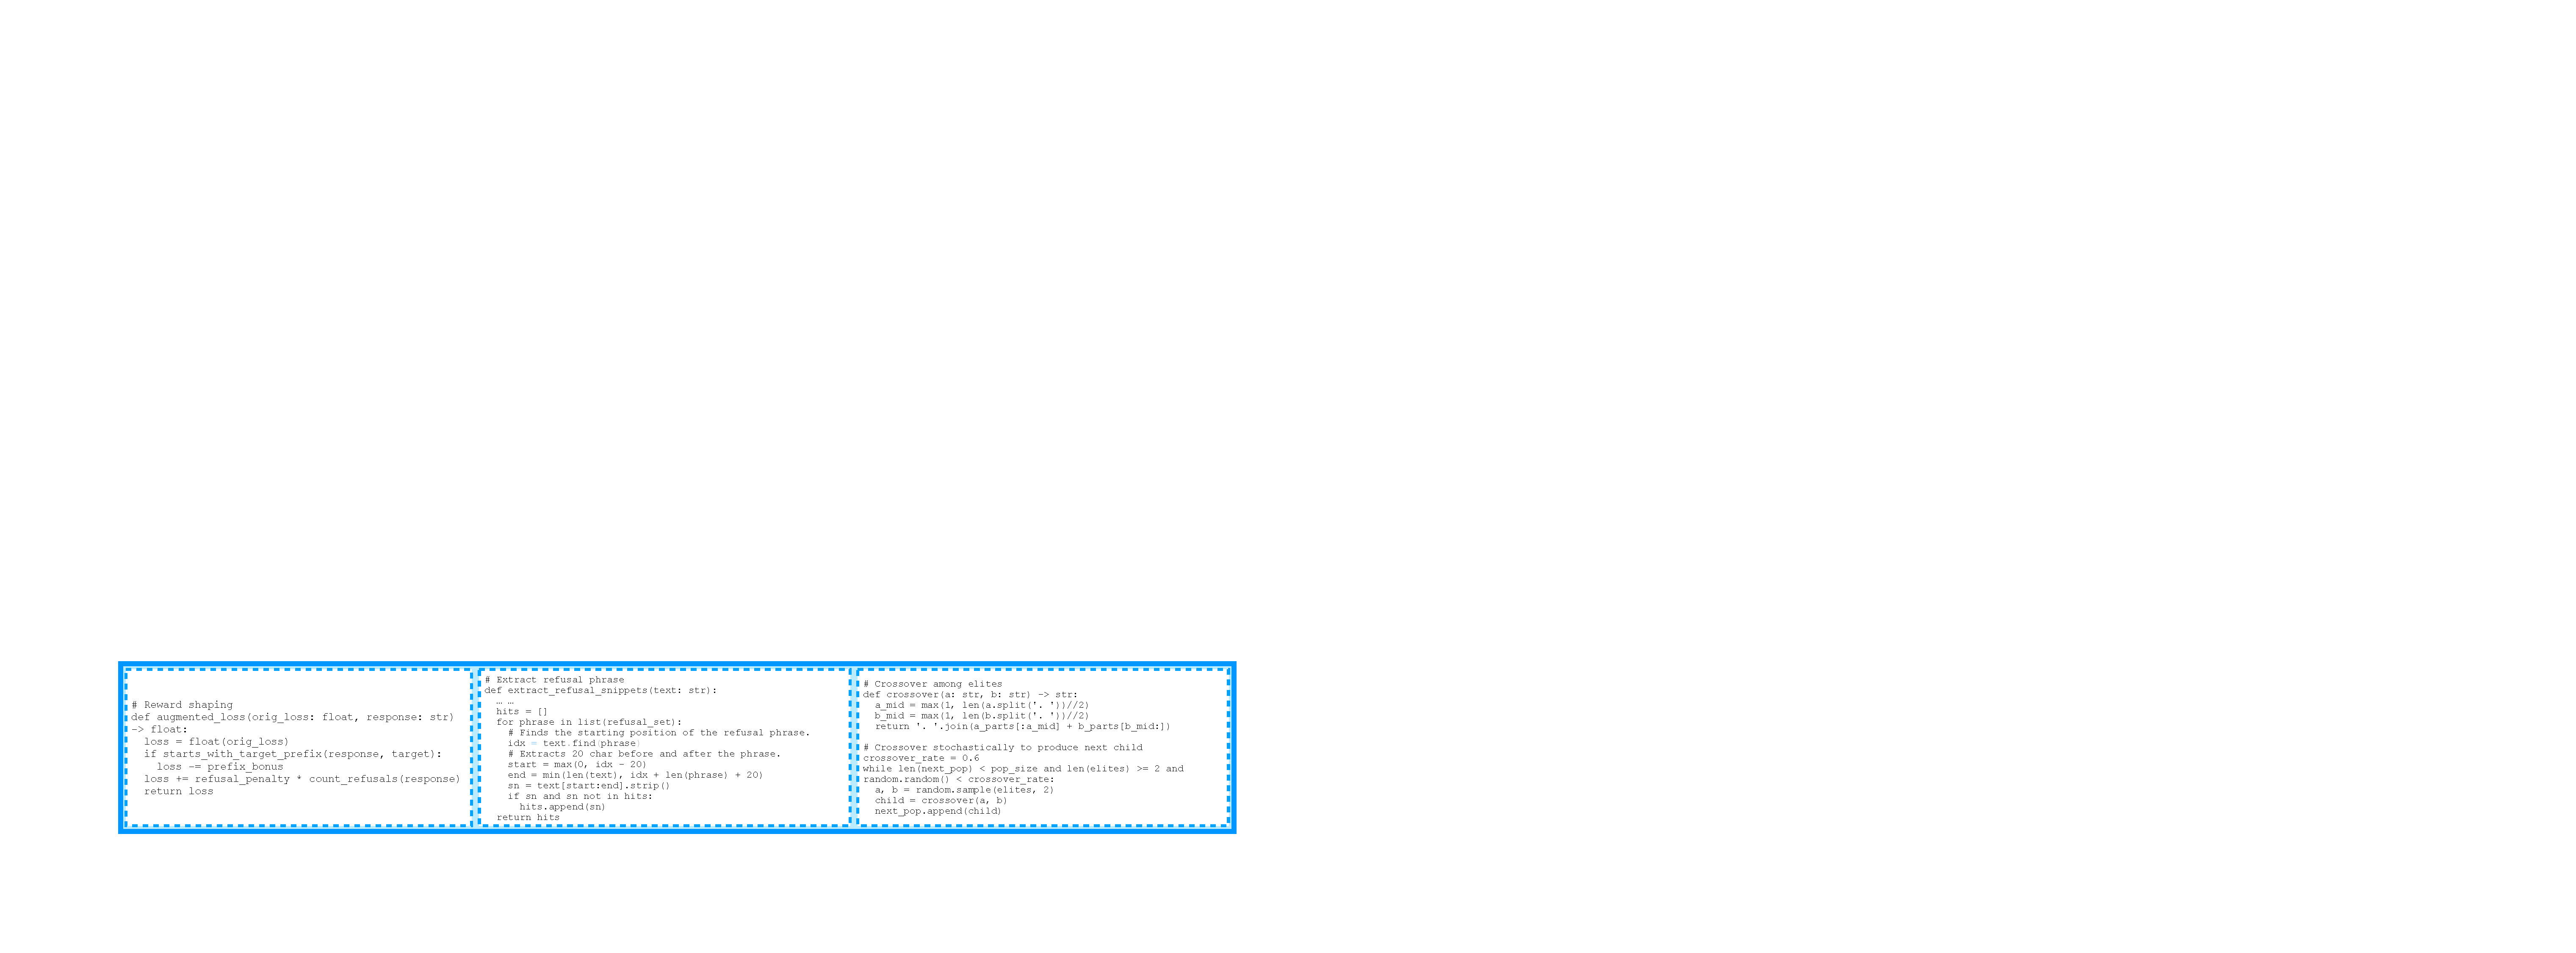
\includegraphics[width=\linewidth]{figure/code_snippet.pdf}
\caption{\textbf{Code snippets produced by \method.} Left: Reward shaping. Center: Refusal suppression. Right: Crossover over elites.}
\label{fig: code snippet}
\vspace{-0.5cm}
\end{figure*}

\textbf{What does the generated system look like?} Upon a closer look into the system that achieves the highest ASR, we found that the meta-agent uncovers \textit{emergent red-teaming strategies} rather than merely recombining existing components from the archive. We present an example agentic system in Appendix \ref{appx: example discovered agentic systems}. Sample code implementing the red-teaming strategies are shown in Figure \ref{fig: code snippet}. Notably, the discovered system effectively leverages its pretrained knowledge about red-teaming research domain into the design, including common jailbreaking strategies from existing literature, such as reward shaping, prefix injection attack and adversarial prompt translation attack \citep{ng1999policy, zou2023universal,li2025decipheringchaosenhancingjailbreak}. It also explored refusal suppression as in \cite{zhou2025don} by recognizing phrases that signal refusal from failed jailbreak attempts (i.e. ``I'm sorry", ``I cannot help") and appends them to a blacklist to explicitly reject responses containing these phrases.

Moreover, the discovered system smartly transfers the notion of evolutionary algorithm into its design choice. It starts with crafting seed instructions drawn from the existing literature of red-teaming. After the first round of attacks, it selects the most effective (``elite") strategies and evolves them by ``crossover" (i.e. combining the first half of one prompt with the second half of another prompt) and ``mutating" (i.e. appending additional protocols) them stochastically. These strategies emerge purely from the automated designs by \method, with zero manual programming.

Altogether, \method~allows the meta agent not only to reuse and improve upon the proposer-and-verifier framework from the baseline, but also to draw inspiration from the ever-growing archive of literature and implement new ideas, which is arguably the most time-consuming part of research.

\textbf{How well do the generated red-teaming systems generalize?} To ensure that the red-teaming systems produced by \method~are indeed generalizable beyond its original setting rather than just reward hacking, we evaluated the generated systems under alternative (1) judge function (2) benchmark datasets (3) proprietary target models.

\textbf{How well do the generated red-teaming systems generalize to different judge functions?} Although the HarmBench classifier is highly aligned with human evaluation, it can occasionally classify harmless responses as jailbreaks and is therefore susceptible to reward hacking. To test whether the produced attacks are robust to the choice of judge function, we evaluate the systems on the held-out test set on both HarmBench and StrongREJECT \citep{souly2024strongrejectjailbreaks}, an alternative judge function that captures fine-grained distinctions in response quality and aligns closely with human assessments of jailbreak quality. As shown in Figure \ref{tab:strongreject_score}, although the original pipeline uses HarmBench to guard its evolution, it outperforms AutoDAN-Turbo by 300\% on Llama-2-7B and by 157\% on Llama-3-8B under StrongREJECT, achieving performance comparable to SOTA methods on proprietary models.

\textbf{Human Study.} Although judge functions provide a practical proxy for jailbreak success, human evaluation remains the gold standard. We randomly sample 200 intention-response pairs and recruit five annotators to assess jailbreak success (details in Appendix \ref{appx: human study}). Our study follows guidelines set by a UW IRB protocol. The results in Table \ref{tab:judge_human_metrics} shows that the HarmBench judge aligns with human judgments overall, achieving strong precision (0.91) and F1-score (0.92). These results confirm that the designed systems produced high-quality jailbreak prompts rather than reward-hacking artifacts.

\begin{table}[htp]
\centering
\scriptsize
\vspace{-0.3cm}
\setlength{\tabcolsep}{4pt}
\resizebox{\textwidth}{!}{%
\begin{tabular}{lccccccccc}
\toprule
\textbf{Method} & \textbf{GPT-3.5-Turbo} & \textbf{GPT-4o} & \textbf{GPT-5.1} & \textbf{GPT-5.2} & \textbf{Sonnet 3.5} & \textbf{Haiku 4.5} & \textbf{DeepSeek-R1} & \textbf{DeepSeek-V3.2} & \textbf{Qwen3-Max} \\
\midrule
% J2             & -   & 94  & -    & -    & 35 & -    & -    & -    & -    \\
% CoP            & -   & -   & -    & -    & 38 & -    & -    & -    & -    \\
% TransferAttack & 80  & -   & -    & -    & -  & -    & -    & -    & -    \\
% AdvReasoning   & -   & 86  & -    & -    & 36 & -    & -    & -    & -    \\
AutoDAN-Turbo  & 90   & -    & 15.5 & 21.5 & 12   & 1.0  & 0.5  & 14.0 & 18.0 \\
PAIR           & 41.0 & 39.0 & 72.5 & 38.5 & 3.0  & 13.0 & 82.5 & 93.0 & 50.0 \\
ActorAttack    & 78.5 & 84.5 & 31.0 & 0.5  & 66.5 & 10.0 & 70.0 & 76.5 & 42.5 \\
Jailbroken     & -    & -    & 29.5 & 7.0  & -    & 0.0  & 99.0 & 95.5 & 21.0 \\
X-Teaming      & -    & 94.3 & 95.5 &  75.5 & \textbf{67.9} & 47.5 & 94.0 & 99.0 & 94.0 \\
\textbf{\method}      & \textbf{100}  & \textbf{100}  & \textbf{100}    & \textbf{88}   & 60   & \textbf{48}  & \textbf{100}   & \textbf{100}  & \textbf{96}  \\
\bottomrule
\end{tabular}%
}
\caption{\textbf{Attack performance on proprietary models on HarmBench.} Baseline numbers are taken directly from \cite{wang2026openrtopensourceredteaming}. Note that the systems generated by \method~were originally designed for Llama2-7B or Qwen3-8B, and are evaluated on the other target models without additional retuning.}
\label{tab: proprietary model}
\vspace{-0.3cm}
\end{table}


% AdvReasoning \citep{sabbaghi2025adversarial} & 60 & 88 & - & 86 & 36 \\
% AutoDAN-Turbo \citep{liu2025autodanturbolifelongagentstrategy} & 36 & 62 & 90 & - & 12 \\
% J2 \citep{kritz2025jailbreaking} & - & - & - & 94 & 35 \\
% CoP \citep{xiong2025cop} & 77 & 71 & - & - & 38 \\
% TransferAttack \citep{yang2025guiding}
\textbf{How well do the generated red-teaming systems generalize to different benchmark datasets?} To ensure that the generated red-teaming systems generalize beyond benchmarks, we additionally evaluated them on AdvBench \citep{chen2022should} and ClearHarm \citep{hollinsworth2025clearharm}. As shown in Figure \ref{fig: across benchmark}, systems designed based on the performance on HarmBench maintain 100\% ASR on both AdvBench and ClearHarm, suggesting that \method~produces robust and query-agnostic attack strategies.

\textbf{How well do the generated red-teaming systems generalize to proprietary models?} As shown in Table \ref{tab: proprietary model}, despite never interacting with closed-weight models during the evolutionary stage, the discovered system achieves 100\% ASR on several of the latest proprietary models, including GPT-5.1, DeepSeek-R1, DeepSeek-V3.2, GPT-4o, and GPT-3.5. It also attains 60\% ASR on Claude Sonnet-3.5 and 44\% on Claude Haiku-4.5, known to be among the most safety-aligned targets that most attack strategies struggle to crack. These results underscore the remarkable transferability and real-world efficacy of \method.

\textbf{Can \method~produce diverse attacks?}
\label{expr: diversity search} Since the objective of red-teaming is to discover as many vulnerabilities of the target LLM as possible, prompt diversity is an important metric in the red-teaming literature alongside ASR \citep{wang2025qualitydiversityredteamingautomatedgeneration}. We therefore leverage generational knowledge to encourage attack diversity by introducing a novelty-based fitness metric that rewards the production of successful yet semantically distinct attacks. Concretely, the novelty of a successful prompt is computed as its average distance to its $k$ nearest neighbors in the embedding space of \texttt{SucceedPromptMemory}, following \citep{rahman2025xteamingmultiturnjailbreaksdefenses}, and the fitness score of a candidate is defined as the mean novelty across all successful prompts it generates. As shown in Figure \ref{fig: diversity search} (middle + right), this approach enables the pipeline to continuously produce novel attacks across generations.